% geometry_and_trigonometry:x02 GDC:NO
\begin{question}
  \hspace*{\fill} [Note Maximale: 6]\par
  \medskip
  \noindent Le diagramme suivant montre le quadrilatère $ABCD$.\par
  \medskip
  \begin{center} % or flushleft or flushright
    \noindent La figure nest pas a l'échelle.\par
    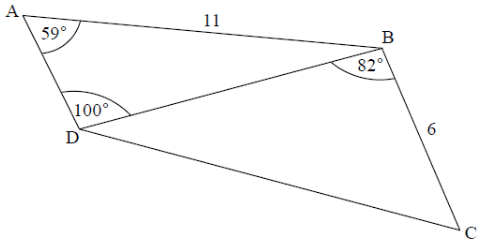
\includegraphics[scale=0.4]{figure_x2}\par
    \noindent $AB = 11cm$, $BC = 6cm$, $\angle\,BAD = 59^\circ$, $\angle\,ADB = 100^\circ$ et $\angle\,CBD = 82^\circ$\par
  \end{center} % or flushleft or flushright

  \begin{enumerate}[label=(\alph*)]
    \item Trouvez DB.\hspace*{\fill} [3]
    \item Trouvez DC.\hspace*{\fill} [3]
  \end{enumerate}
\end{question}
